\section{Специальный раздел}
\label{sec:special}

\subsection{Требования к разрабатываемой системе}

В данном разделе представлены ключевые аспекты разработки системы токенизации дипломов на основе блокчейн-технологий для цифровой верификации и децентрализованного хранения образовательных достижений. 

Требования к разрабатываемому программному продукту описывают набор параметров и характеристик, необходимых для полноценного функционирования системы. Они определяют функциональность системы, а также поведение и условия, необходимые для стабильной работы. Такие требования классифицируются на функциональные и нефункциональные~\cite{bib:func_and_nf_req}.

\hyperref[subsec:func_req]{Функциональные требования} определяют конкретные задачи и операции, которые должна выполнять система для достижения заранее заданных целей. Описывается поведение в различных сценариях, включая процессы обработки данных, взаимодействие с пользователями, а также выполнение основных и дополнительных функций. Функциональные требования являются измеримыми и точно определенными; их выполнение можно однозначно проверить с помощью тестирования. Они играют важную роль в разработке систем, так как непосредственно влияют на архитектуру и проектные решения.

\hyperref[subsec:nonfunc_req]{Нефункциональные требования} формулируют качественные атрибуты системы, которые не влияют непосредственно на конкретные действия, но определяют общее качество и условия работы. Они включают производительность, безопасность, доступность, удобство использования, совместимость, масштабируемость, а также методики к тестированию и документации. Эти требования устанавливают ограничения и стандарты, которым должен соответствовать программный продукт, чтобы удовлетворять ожидания пользователей и обеспечивать надёжную и стабильную работу. Нефункциональные требования критически важны для обеспечения высокого уровня пользовательского опыта и управляемости системы на протяжении всего срока эксплуатации.

Функциональные и нефункциональные требования занимают важное место в процессе разработки продукта. Они формируют фундамент для проектирования, реализации и последующего тестирования системы. Без точно сформулированных задач создание эффективного и надежного программного продукта, отвечающего  потребностям пользователей и бизнес-задачам, становится невозможным~\cite{bib:app_req}.

\subsubsection{Функциональные требования}
\label{subsec:func_req}

В рамках подраздела рассматриваются функциональные требования к разрабатываемому программному продукту:

\begin{enumerate}
    \item Коллекции дипломов:
    \begin{enumerate}
        \item должна быть возможность создания общей коллекции для каждого образовательного учреждения, которая будет агрегировать все подколлекции выпусков в виде дополнительных токенов;
        \item коллекция должна служить отдельным регистром для выпускаемых дипломов, позволяя классифицировать их по годам выпуска, специализациям или другим параметрам;
        \item каждая коллекция должна иметь уникальный идентификатор в блокчейне и быть доступной для запросов и проверок через публичные функции смарт-контракта.
    \end{enumerate}
    \item Дипломы пользователей:
    \begin{enumerate}
        \item cоздание диплома должно происходить через смарт-контракты, гарантируя уникальный токена для каждого пользователя;
        \item дипломы должны связываться с уникальными данными студентов, такими как специализация и уровень образования;
        \item при создании диплома должна быть возможность указать дополнительные образовательные достижения студента.
    \end{enumerate}
    \item Защита персональных данных~\cite{bib:152fz}:
    \begin{enumerate}
        \item персональные данные, связанные со студентом, например имя или индивидуальный номер студента, должны быть преобразованы с применением однонаправленных криптографических алгоритмов;
        \item при выпуске диплома, данные, неявно идентифицирующие пользователя должны быть минимизированы.
    \end{enumerate}
    \item Мультиподпись:
    \begin{enumerate}
        \item при выпуске каждого диплома требуется подтверждение от нескольких уполномоченных лиц, например, представителей факультета и деканата;
        \item необходимо наличие технической поддержки мультиподписи в смарт-контрактах для обеспечения контроля и одобрения выпуска дипломов.
    \end{enumerate}
    \item Верификация диплома:
    \begin{enumerate}
        \item система должна предоставлять механизмы для публичной проверки подлинности дипломов, включая доступ к хешам;
        \item верификация должна быть простой и не требовать сложных технических знаний от пользователей, делая процесс доступным для работодателей и образовательных учреждений;
        \item должна быть возможность подлинность диплома как через систему, так и самостоятельно.
    \end{enumerate}
    \item Интерфейс пользователя:
    \begin{enumerate}
        \item пользователям должен быть доступен Telegram-бот с возможностью получения и проверки диплома;
        \item Telegram-бот должен предоставлять функции для регистрации пользователей, запросов на выпуск дипломов и их верификации.
    \end{enumerate}
    \item Поддержка кастодиальных и некастодиальных кошельков:
    \begin{enumerate}
        \item пользователи должны иметь возможность выбирать между самостоятельным управлением своими ключами или использованием кастодиальных сервисов для хранения ключей;
        \item система должна интегрироваться с платформой thirdweb для обеспечения поддержки различных типов авторизации и аутентификации.
    \end{enumerate}
    \item Обработка запросов через собственный узел удаленного вызова процедур (Remote procedure call, RPC):
    \begin{enumerate}
        \item использование собственного RPC-узла должно увеличить скорость и надежность транзакций, минимизируя зависимость от сторонних провайдеров;
        \item настройка RPC узла должна быть оптимизирована для обработки большого количества запросов, обеспечивая стабильность и высокую производительность системы.
    \end{enumerate}
\end{enumerate}

\subsubsection{Нефункциональные требования}
\label{subsec:nonfunc_req}

Для обеспечения полноценной работоспособности и надежности разрабатываемой системы токенизации дипломов на базе блокчейн-технологий для цифровой верификации и децентрализованного хранения образовательных достижений, особое внимание уделяется формулировке нефункциональных требований. Они задают качественные стандарты для архитектуры системы, определяя общую производительность, безопасность, доступность и удобство использования. Наиболее важными из них являются:

\begin{itemize}
    \item cистема должна использовать передовые методы криптографической защиты. Механизмы мультиподписи должны быть реализованы так, чтобы обеспечить необходимый уровень доверия и верификации среди всех участвующих сторон;
    \item система должна обеспечивать стабильную и непрерывную работу. Это критически важно для пользователей, которые могут нуждаться в проверке подлинности достижений в любое время из любой точки мира;
    \item система должна обеспечивать быстрое время ответа и высокую пропускную способность при обработке транзакций, что особенно важно в периоды высоких нагрузок, например, во время выпускных экзаменов и вручения дипломов;
    \item система должна быть совместима с различными блокчейнами, основанными на EVM (Ethereum Virtual Machine), особенно с сетями Polygon и Siberium, выбранными в аналитическом разделе. Важно предусмотреть возможность интеграции с другими образовательными и информационными системами через стандартизированные двоичные интерфейсы приложения (Application Binary Interface, ABI)~\cite{bib:sc_abi};
    \item клиентский интерфейс должен быть простым и интуитивно понятным, чтобы пользователи всех уровней могли легко управлять своими дипломами и проводить верификацию без дополнительных сложностей.
\end{itemize}

Реализация этих нефункциональных требований позволит создать систему, которая не только технически продвинута, но и удобна в использовании, безопасна и надежна, что обеспечит долгосрочную устойчивость системы и её способность адаптироваться к изменяющимся технологическим и операционным условиям.

\subsection{Проектирование системы}

В рамках разработки системы токенизации дипломов на основе блокчейн-технологий, основной акцент делается на проектировании архитектуры, которая позволит обеспечить цифровую верификацию и децентрализованное хранение образовательных достижений.

Упрощённая диаграмма использование, на рисунке~\ref{fig:uscs}, показывает варианты использования и основные функции системы, включая их доступность для различных типов пользователей.

\begin{figure}[H]
	\centering
	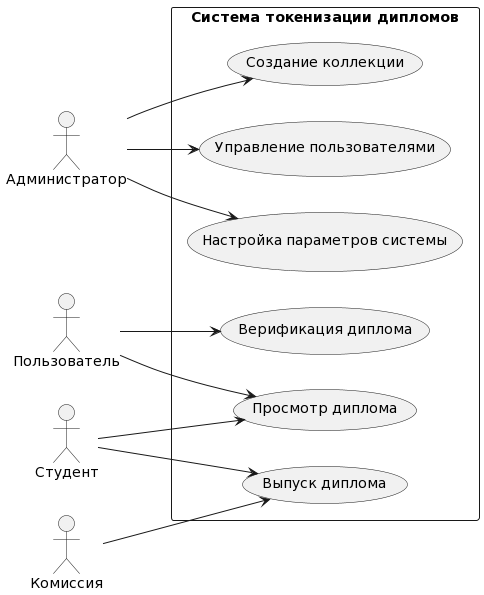
\includegraphics[width=.6\textwidth]{images/uscs.png}
	\parskip=6pt
	\caption{Упрощённая диаграмма использования}
	\label{fig:uscs}
\end{figure}

Система токенизации дипломов включает четыре категории пользователей: Администратор, Пользователь, Студент и Комиссия, каждая из которых выполняет свои специфические функции. Администратор отвечает за создание коллекций дипломов, управление пользователями и настройку параметров системы, обеспечивая организацию и поддержание целостности базы данных дипломов.

Комиссия участвует в процессе выпуска дипломов, проверяя и верифицируя представленные студентами данные. Пользователи могут проверять подлинность дипломов и просматривать их, что обеспечивает прозрачность и достоверность представленной информации. Такая структура системы позволяет эффективно управлять дипломами, от их создания до проверки и просмотра.

Проектирование данной системы включает создание нескольких ключевых компонентов, отображённых на рисунке~\ref{fig:sys_arch}.

\begin{figure}[H]
	\centering
	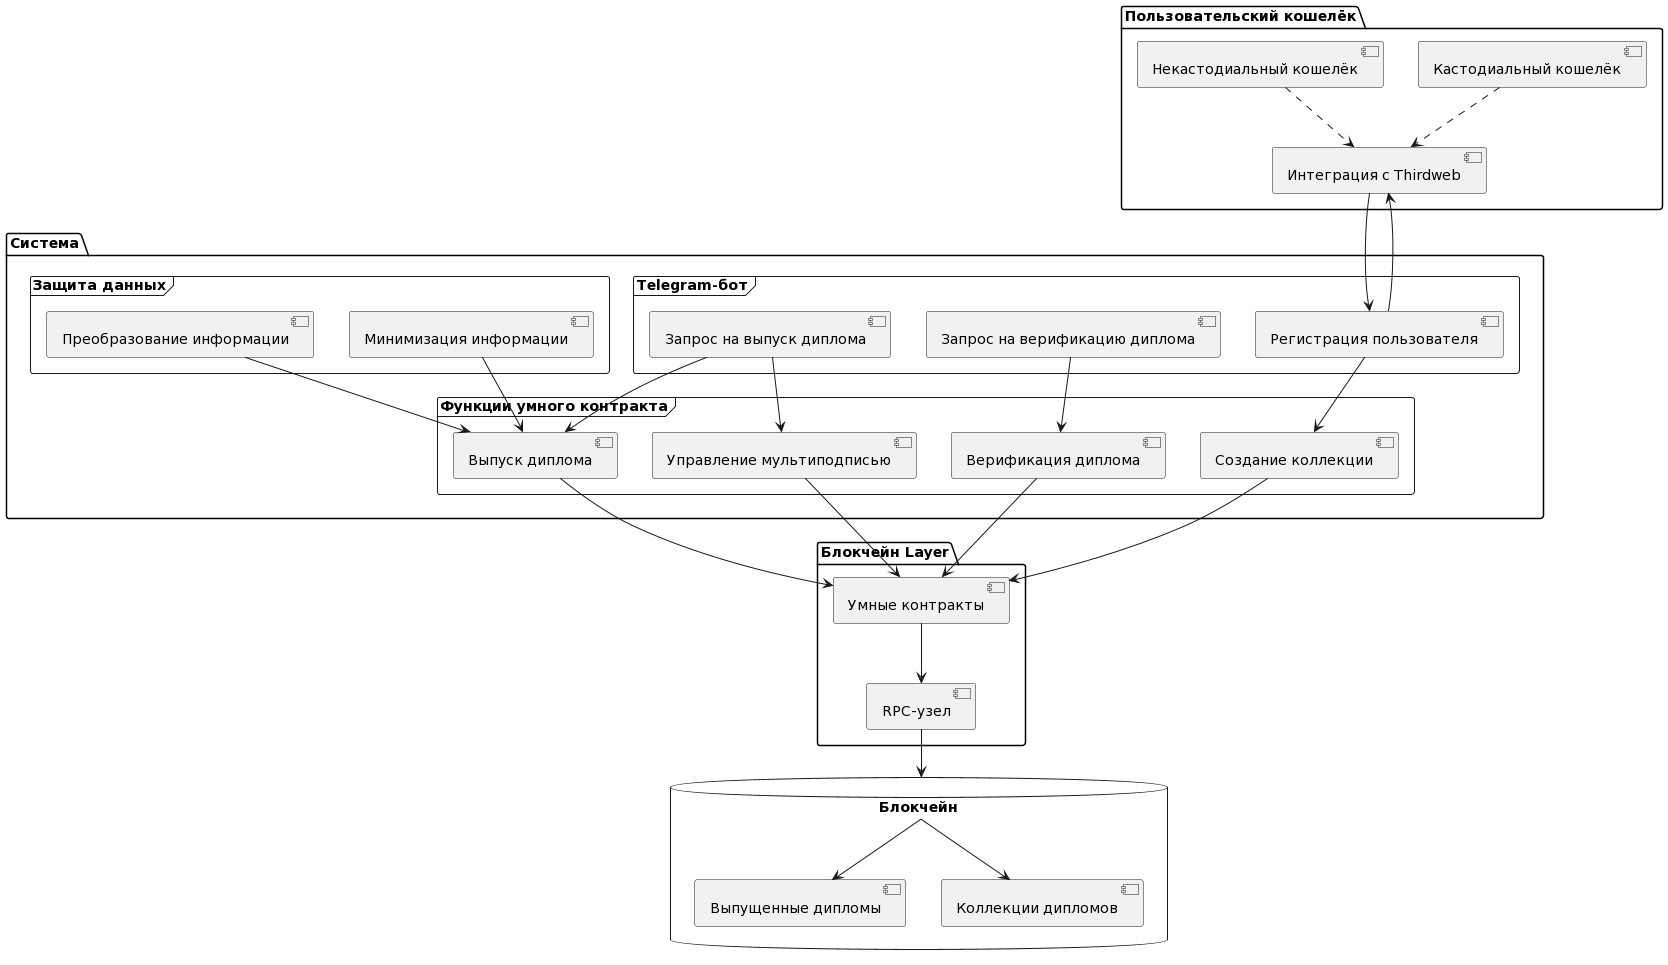
\includegraphics[width=.9\textwidth]{images/sys_arch.png}
	\parskip=6pt
	\caption{Общая схема архитектуры системы цифровых дипломов}
	\label{fig:sys_arch}
\end{figure}

В общем виде система состоит из следующих компонентов:

\begin{itemize}
    \item основа системы, которая управляет логикой создания, хранения и верификации цифровых дипломов. Смарт-контракты разрабатываются таким образом, чтобы обеспечить выполнение всех операций без возможности вмешательства сторонних лиц после их развертывания на блокчейне;
    \item использование блокчейн-платформ, таких как Ethereum, Polygon, и Siberium, для обеспечения надежности и децентрализации данных. Это включает в себя разработку уникальных идентификаторов для каждого диплома и механизмов их токенизации;
    \item применение криптографических методов для защиты персональной информации студентов, включая хеширование и шифрование данных. Это критически важно для соответствия нормам о защите персональных данных, таких как <<Общий регламент по защите данных>> (General Data Protection Regulation, GDPR) и Федеральному закону <<О персональных данных>> №152-ФЗ~\cite{bib:152fz};
    \item реализация механизма мультиподписи для усиления доверия к процессу выпуска дипломов. Каждый диплом требует подтверждения от нескольких уполномоченных лиц учебного заведения, что усложняет возможность его несанкционированной выдачи;
    \item разработка пользовательского интерфейса через Telegram-бота, который облегчает доступ к функциям системы для конечных пользователей. Бот позволяет регистрироваться в системе, запрашивать выпуск и верификацию дипломов, а также получать уведомления о статусе своих запросов;
    \item оптимизация обработки запросов в блокчейне с использованием собственного RPC-узла, что увеличивает скорость обработки данных и снижает зависимость от сторонних сервисов.
\end{itemize}

Диаграмма активности, на рисунке~\ref{fig:ifcs}, показывает процесс выпуска диплома от начала до конца, включая все основные шаги и условные переходы.
\begin{figure}[H]
	\centering
	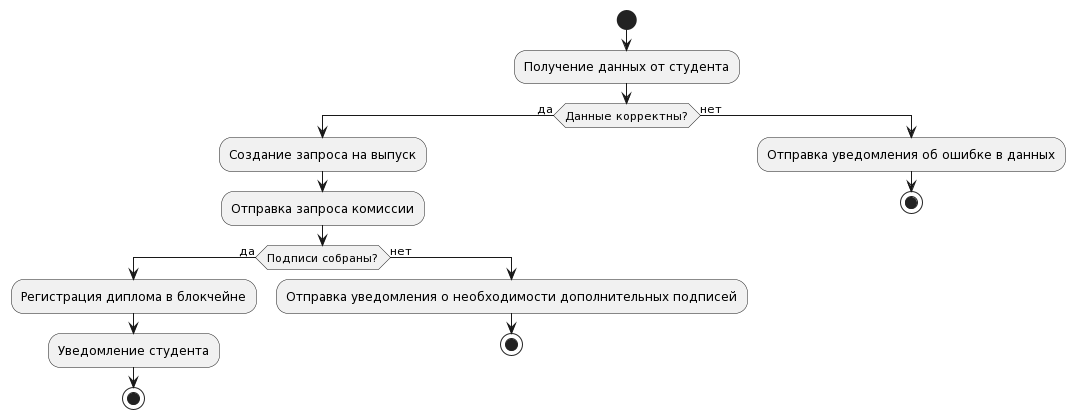
\includegraphics[width=.9\textwidth]{images/ifcs.png}
	\parskip=6pt
	\caption{Общая схема архитектуры системы цифровых дипломов}
	\label{fig:ifcs}
\end{figure}

Действия в системе начинаются с получения данных от студента. Затем проводится проверка корректности полученных данных. Если данные корректны, формируется запрос на выпуск диплома, который затем отправляется комиссии для получения подписей. Если все необходимые подписи собраны, диплом регистрируется в блокчейне, после чего студенту приходит уведомление о завершении процесса. Если подписи не собраны, студент получает уведомление об ошибке или отказе.

В случае, если данные, предоставленные студентом, некорректны, студенту отправляется уведомление об ошибке в данных, и процесс прекращается до устранения ошибок.

\subsubsection{Архитектура базы данных и Telegram-бота для системы}

В данной части описывается структура базы данных и архитектура Telegram-бота, разработанные для системы токенизации дипломов. Эти компоненты являются ключевыми для обеспечения функциональности системы, включая регистрацию и аутентификацию пользователей, обработку запросов на выпуск дипломов и управление уведомлениями.

Визуализация структуры базы данных и функций Telegram-бота представлена на рисунке~\ref{fig:tg_dc}, которая помогает понять взаимосвязи и зависимости между различными компонентами системы.

\begin{figure}[H]
	\centering
	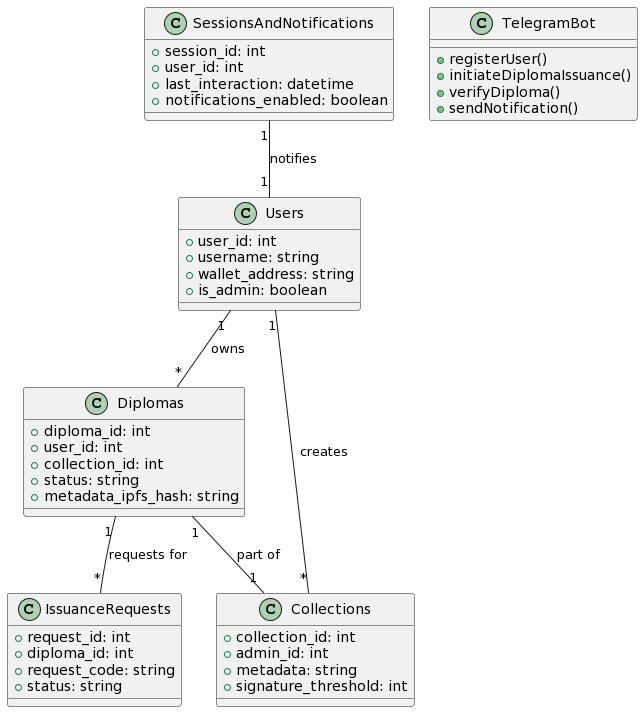
\includegraphics[width=.9\textwidth]{images/tg_dc.png}
	\parskip=6pt
	\caption{Диаграмма классов Telegram-бота}
	\label{fig:tg_dc}
\end{figure}

База данных системы разделена на несколько основных сущностей:

\begin{enumerate}
    \item \textit{Пользователи (Users):} таблица содержит информацию о пользователях системы. Каждый пользователь идентифицируется уникальным идентификатором и связан с именем пользователя Telegram, а также адресом его блокчейн-кошелька. Специальный атрибут определяет, имеет ли пользователь административные права для управления системой.
    \item \textit{Дипломы (Diplomas):} включает записи о каждом выпущенном дипломе, связанные с пользователем через его идентификатор и с коллекцией через идентификатор коллекции. Статус диплома отслеживает его текущее состояние в системе, а метаданные содержат ссылку на диплом в IPFS (InterPlanetary File System)~\cite{bib:ipfs_is}.
    \item \textit{Коллекции (Collections):} содержит информацию о коллекциях дипломов, созданных администраторами. Каждая коллекция имеет уникальный идентификатор, администратора, связанного с коллекцией, и метаданные, которые описывают коллекцию и условия её использования.
    \item \textit{Запросы на выпуск (Issuance Requests):} таблица, отражающая запросы на выпуск дипломов, связанные с конкретными дипломами и содержащие уникальный код, который используется для активации процесса в Telegram-боте.
    \item \textit{Сессии и уведомления (Sessions and Notifications):} управляет сессиями пользователей и их настройками уведомлений, что позволяет эффективно распространять информацию о статусе запросов и дипломов.
\end{enumerate}

\subsubsection{Процесс выпуска цифрового диплома}

Процесс выпуска цифрового диплома начинается с администратора (университета или организации, выдающей диплом), который создаёт коллекцию для дипломов в блокчейне. Этот процесс включает шаги, указанные на рисунке~\ref{fig:diploma_issue}.

\begin{figure}[H]
	\centering
	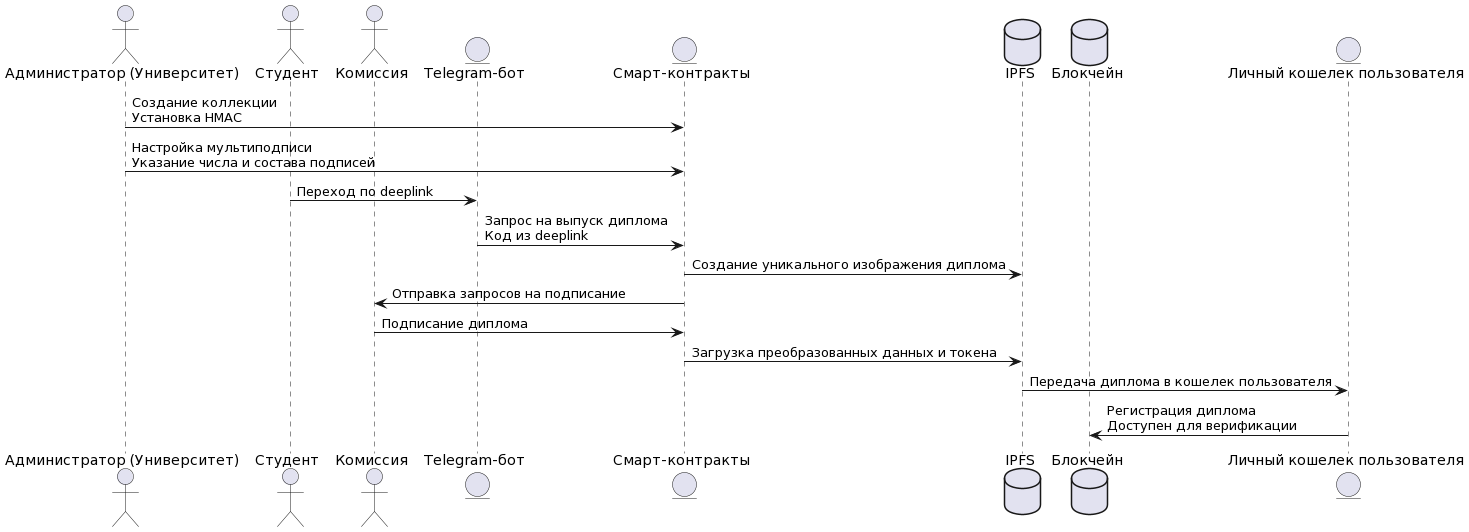
\includegraphics[width=.9\textwidth]{images/diploma_issue.png}
	\parskip=6pt
	\caption{Диаграмма последовательности выпуска цифрового диплома}
	\label{fig:diploma_issue}
\end{figure}

При подробном рассмотрении можно выделить основные этапы:

\begin{enumerate}
    \item Создание коллекции:
    \begin{enumerate}
        \item администратор (обычно представитель университета) инициирует создание новой коллекции дипломов;
        \item метаданные коллекции размещаются в IPFS, делая их доступными для общего просмотра и использования;
        \item определяется количество необходимых подписей для выпуска диплома, а также состав комиссии, которая будет подписывать дипломы;
        \item устанавливается процентное соотношение подписей, требуемых для завершения процесса выпуска диплома.
    \end{enumerate}
    \item Создание диплома:
    \begin{enumerate}
        \item на основе учебных достижений, специальности и оценки за диплом создаётся уникальное изображение, которое визуализирует достижения студента;
        \item также формируются метаданные токена, которые помогают указать дополнительную информацию о дипломе.
    \end{enumerate}
    \item Защита дипломной работы и выпуск диплома:
    \begin{enumerate}
        \item после успешной защиты дипломной работы, студент переходит по специальной ссылке (deeplink) в Telegram-бот, который распознаёт код из ссылка и инициирует процесс выпуска диплома.
    \end{enumerate}
    \item Подписание диплома комиссией:
    \begin{enumerate}
        \item каждому члену комиссии отправляется запрос на подписание диплома через их блокчейн-кошельки. Уведомления о необходимости подписи также поступают через Telegram;
        \item как только требуемое количество членов комиссии подписывает диплом, преобразованные данные и сам токен загружаются в IPFS для хранения метаданных.
    \end{enumerate}
    \item Размещение диплома в кошельке пользователя:
    \begin{enumerate}
        \item после подписания и загрузки в IPFS, цифровой диплом переходит в личный кошелёк пользователя, где он становится доступным для публичной проверки и использования.
    \end{enumerate}
\end{enumerate}

\subsubsection{Процесс преобразования данных пользовтаелей}

Процесс преобразования данных пользователя в системе токенизации дипломов начинается с получения основной информации от пользователя, которая затем обрабатывается для обеспечения её конфиденциальности с использованием криптографических методов, указанных на рисунке~\ref{fig:data_proc}.

\begin{figure}[H]
	\centering
	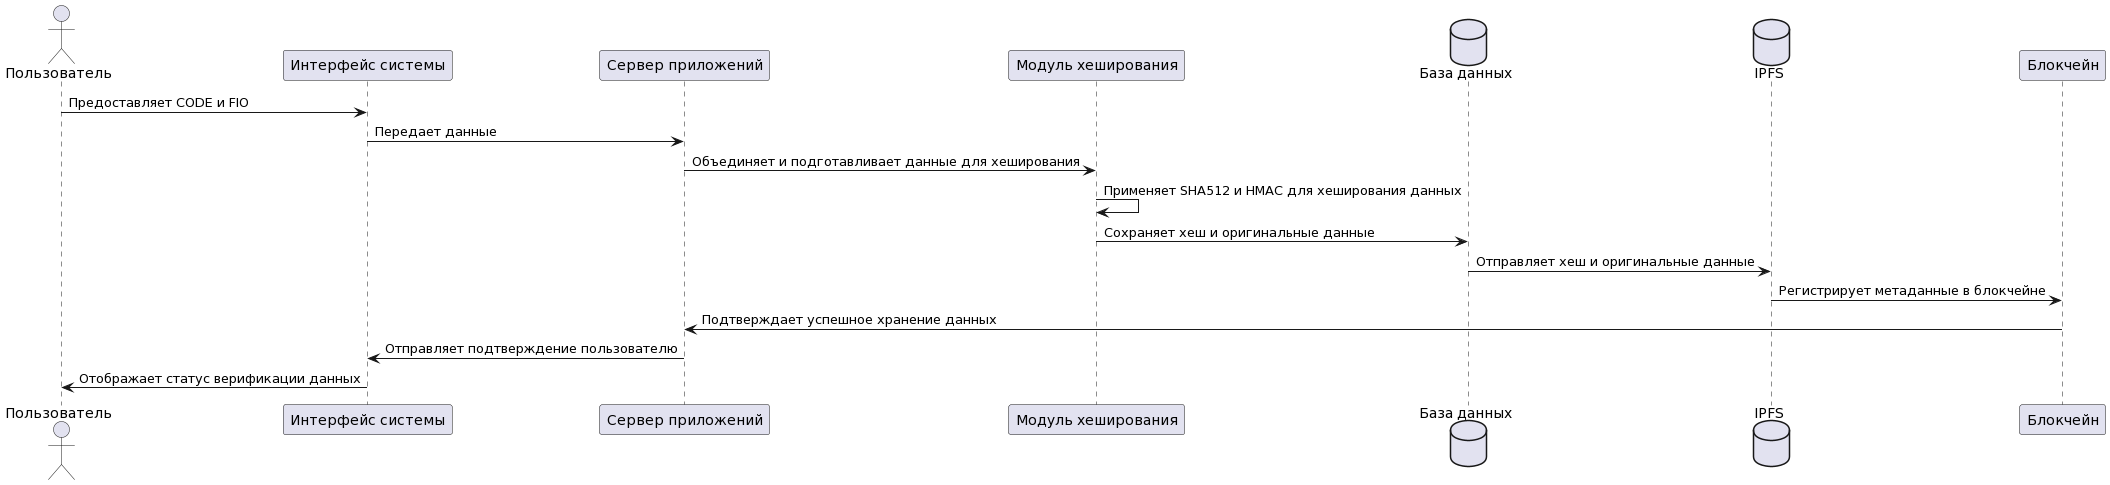
\includegraphics[width=.9\textwidth]{images/data_proc.png}
	\parskip=6pt
	\caption{Диаграмма последовательности преобразования данных}
	\label{fig:data_proc}
\end{figure}

В системе токенизации дипломов процесс верификации данных начинается с взаимодействия пользователя с интерфейсом системы, где он предоставляет свои идентификационные данные, включая уникальный код и ФИО. Для обеспечения безопасности и целостности данных, клиент использует модуль хеширования, который применяет криптографические алгоритмы SHA512 и HMAC. После сохранения, данные отправляются в распределенную файловую систему IPFS.

\subsubsection{Процесс верификации цифровых дипломов}

Процесс верификации, на рисунке~\ref{fig:diploma_verif}, цифровых дипломов в системе токенизации дипломов на блокчейн-технологии позволяет проверить подлинность диплома и идентифицировать принадлежность его конкретному пользователю. Этот процесс важен как для работодателей, так и для образовательных учреждений, стремящихся подтвердить квалификацию кандидатов.

\begin{figure}[H]
	\centering
	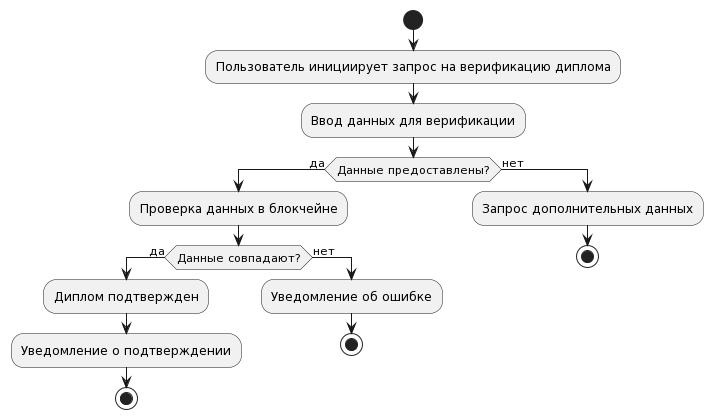
\includegraphics[width=.9\textwidth]{images/diploma_verif.png}
	\parskip=6pt
	\caption{Диаграмма последовательности преобразования данных}
	\label{fig:diploma_verif}
\end{figure}

Процесс верификации начинается запроса на проверку подлинности диплома. Пользователь вводит необходимые данные для верификации через интерфейс системы. После ввода данных система проверяет их наличие. Если хеши совпадают, диплом считается подтвержденным, и пользователь получает уведомление о подтверждении подлинности диплома. Этот шаг гарантирует, что диплом является аутентичным и соответствует записи.

Диаграмма последовательности, на рисунке~\ref{fig:diploma_verif_uscs}, иллюстрирует процесс с момента инициации запроса пользователем до получения результатов верификации. В зависимости от результата проверки в блокчейне, пользователь получает уведомление либо о подтверждении подлинности диплома, либо о наличии ошибки.

\begin{figure}[H]
	\centering
	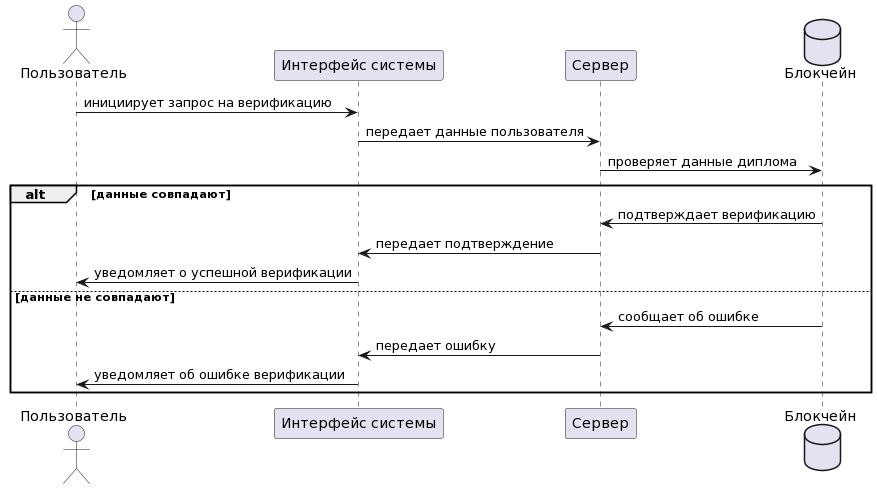
\includegraphics[width=.9\textwidth]{images/diploma_verif_uscs.png}
	\parskip=6pt
	\caption{Диаграмма последовательности преобразования данных}
	\label{fig:diploma_verif_uscs}
\end{figure}

